% Figure 1: The Architecture of Formlaere — composite 4-panel
% A+B from Python (PDF), C+D from TikZ

\begin{figure*}[!t]
\centering

% ── TOP ROW: Data panels ──
\begin{minipage}[t]{0.48\textwidth}
\centering
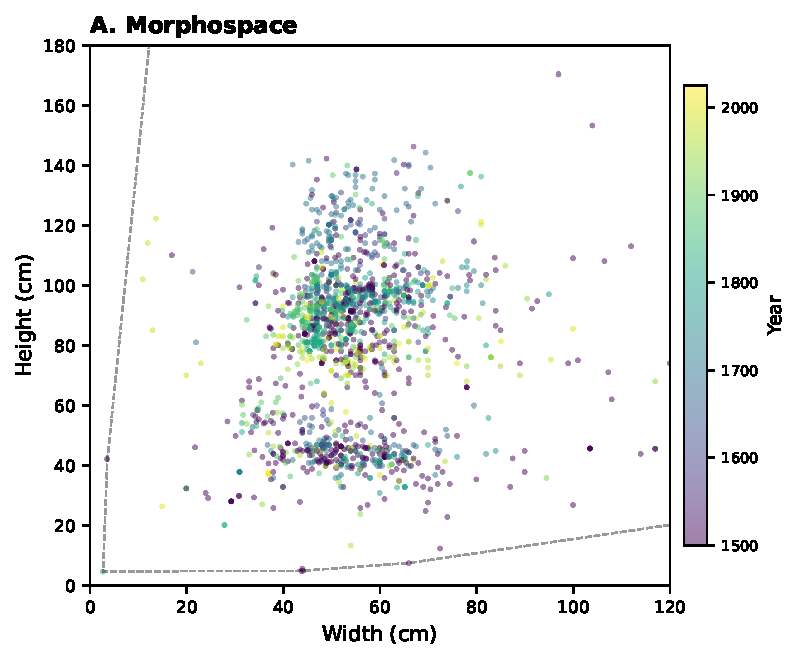
\includegraphics[width=\textwidth]{figures/fig-2-morphospace.pdf}
\end{minipage}%
\hfill
\begin{minipage}[t]{0.48\textwidth}
\centering
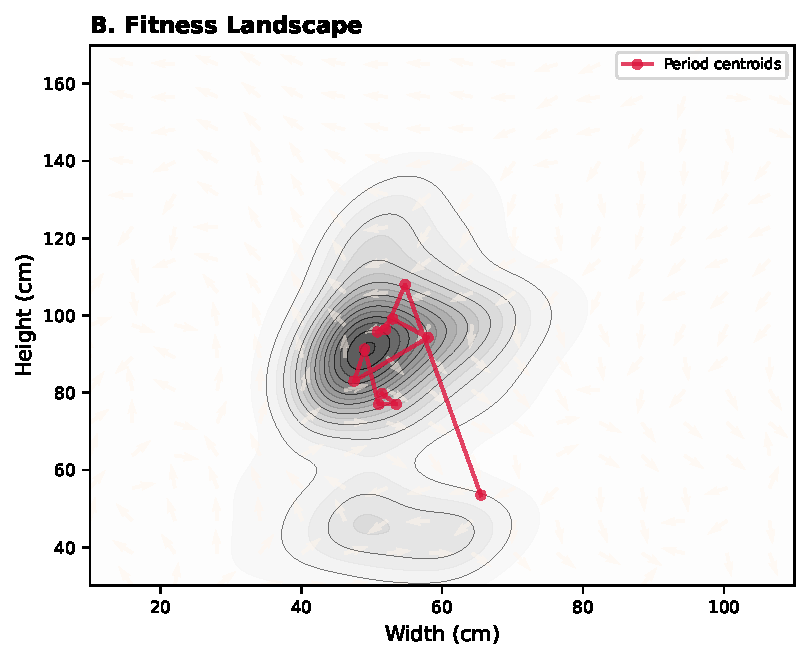
\includegraphics[width=\textwidth]{figures/fig-3-landscape.pdf}
\end{minipage}

\vspace{6pt}

% ── BOTTOM ROW: Structural panels ──
\begin{minipage}[t]{0.48\textwidth}
\centering
{\small\bfseries C.\enspace Multi-Scale Agency}\\[4pt]
\begin{tikzpicture}[
  scale=0.72, transform shape,
  cone/.style={draw=black!60, fill=black!4, thick},
  agent/.style={font=\scriptsize, text=black},
  label/.style={font=\tiny, text=black!70},
  >={Stealth[length=3pt]}
]
\draw[cone, fill=black!3] (-3.0, 0) -- (0, 4.8) -- (3.0, 0) -- cycle;
\node[agent, anchor=west] at (2.1, 0.3) {Market};
\node[label, anchor=west] at (2.1, 0.0) {decade};
\draw[cone, fill=black!5] (-2.2, 0) -- (0, 4.8) -- (2.2, 0) -- cycle;
\node[agent, anchor=west] at (1.5, 0.9) {Designer};
\node[label, anchor=west] at (1.5, 0.6) {month};
\draw[cone, fill=black!7] (-1.5, 0) -- (0, 4.8) -- (1.5, 0) -- cycle;
\node[agent, anchor=west] at (0.9, 1.6) {Tool};
\node[label, anchor=west] at (0.9, 1.3) {hour};
\draw[cone, fill=black!9] (-0.9, 0) -- (0, 4.8) -- (0.9, 0) -- cycle;
\node[agent, anchor=west] at (0.4, 2.4) {Material};
\node[label, anchor=west] at (0.4, 2.1) {minute};
\draw[cone, fill=black!12] (-0.35, 0) -- (0, 4.8) -- (0.35, 0) -- cycle;
\node[agent, anchor=east] at (-0.05, 3.2) {Cell};
\node[label, anchor=east] at (-0.05, 2.9) {ms};
\filldraw[black] (0, 4.8) circle (2pt);
\draw[decorate, decoration={brace, amplitude=4pt, mirror}, black!50]
  (-3.2, -0.1) -- (-3.2, 4.9) node[midway, left=6pt, font=\scriptsize, text=black!70, rotate=90, anchor=south] {cognitive cone $C(A)$};
\draw[<->, black!50] (-3.0, -0.5) -- (3.0, -0.5)
  node[midway, below, font=\scriptsize] {care $= \dim C(A)$};
\end{tikzpicture}
\end{minipage}%
\hfill
\begin{minipage}[t]{0.48\textwidth}
\centering
{\small\bfseries D.\enspace The Synthesis}\\[4pt]
\begin{tikzpicture}[
  scale=0.72, transform shape,
  box/.style={draw=black, rounded corners=3pt, minimum width=26mm, minimum height=8mm,
              font=\small, align=center, thick},
  pillar/.style={draw=#1, fill=#1!8, rounded corners=2pt, minimum width=22mm,
                 minimum height=6mm, font=\scriptsize, align=center},
  >={Stealth[length=3pt]}
]
\node[pillar=teal] (syn) at (-2.4, 4.2) {\textsc{Syntax}\\[-1pt]\tiny Stiny};
\node[pillar=orange!80!black] (log) at (0, 4.2) {\textsc{Logic}\\[-1pt]\tiny Hatchuel \& Weil};
\node[pillar=purple!70!black] (dyn) at (2.4, 4.2) {\textsc{Dynamics}\\[-1pt]\tiny Levin};
\node[box, minimum width=68mm, fill=black!5] (eq) at (0, 2.6)
  {$\mathrm{Form} = SG\!\left(\nabla_{C(A)}\, L(c,\,t)\right)$};
\node[box, fill=teal!8, draw=teal, minimum width=20mm] (sg) at (-2.4, 1.0) {$SG$\\[-2pt]\tiny grammar};
\node[box, fill=orange!8, draw=orange!80!black, minimum width=20mm] (lc) at (0, 1.0) {$L(c,t)$\\[-2pt]\tiny landscape};
\node[box, fill=purple!8, draw=purple!70!black, minimum width=20mm] (ca) at (2.4, 1.0) {$\nabla_{C(A)}$\\[-2pt]\tiny cone};
\node[box, fill=black!8, minimum width=46mm] (form) at (0, -0.4)
  {\textbf{Form} $x \in M(c)$};
\node[font=\small\itshape, text=black!80] (care) at (0, -1.4)
  {care $= \dim C(A)$};
\draw[->, thick, teal] (syn) -- (eq);
\draw[->, thick, orange!80!black] (log) -- (eq);
\draw[->, thick, purple!70!black] (dyn) -- (eq);
\draw[->, thick, teal] (eq) -- (sg);
\draw[->, thick, orange!80!black] (eq) -- (lc);
\draw[->, thick, purple!70!black] (eq) -- (ca);
\draw[->, thick] (sg) -- (form);
\draw[->, thick] (lc) -- (form);
\draw[->, thick] (ca) -- (form);
\draw[->, dashed, thick, black!50] (form.east) -- ++(1.0, 0) |- (lc.east)
  node[pos=0.25, right, font=\tiny, text=black!60] {$K$ expands};
\end{tikzpicture}
\end{minipage}

\caption{The architecture of \formlaere{}. \textbf{A}: 1,662 European chairs projected into morphospace (width $\times$ height); color encodes date. \textbf{B}: Fitness landscape as kernel density estimate with gradient vector field and period centroid trajectory (red). \textbf{C}: Nested cognitive cones across five competence scales; cone width corresponds to care dimensionality. \textbf{D}: The synthesis equation; three source traditions converge on the core equation; dashed arrow shows $K$-expansion feedback.}
\label{fig:architecture}
\end{figure*}
